%% conclusion.tex
%%

%% ==============================
\chapter{Conclusions and future work}
\label{ch:conclusion}
%% ==============================

\section{The ``Heisenberg Effect''}
\label{sec:conclusion:heisenberg}

The analysis of the collected data in section~\ref{sec:evaluation:indications} shows that there is an effect, which cannot be explained by hand tremor or device jitter, resulting in a worse pointing accuracy and maybe even a worse throughput. This effect shows many similarities to the described ``Heisenberg Effect'' by Bowman~\cite{bowman_using_2001} and Kopper et al.~\cite{kopper_human_2010}, like the occured offset in direction of the pressed trigger, demonstrated in Figure~\ref{fig:plot}. 

The incentive to this work was to show evidence for the ``Heisenberg Effect'', analyze its effects and give a good basis for compensating it. The results which are shown in this thesis leap to the conclusion, that the ``Heisenberg Effect'' exists and has a bigger impact on pointing accuracy and throughput as previously thought.

\section{Compensation for the ``Heisenberg Effect'' and Implications for future work}
\label{sec:conclusion:compensation_future_work}

\begin{figure}[h]
    \centering
    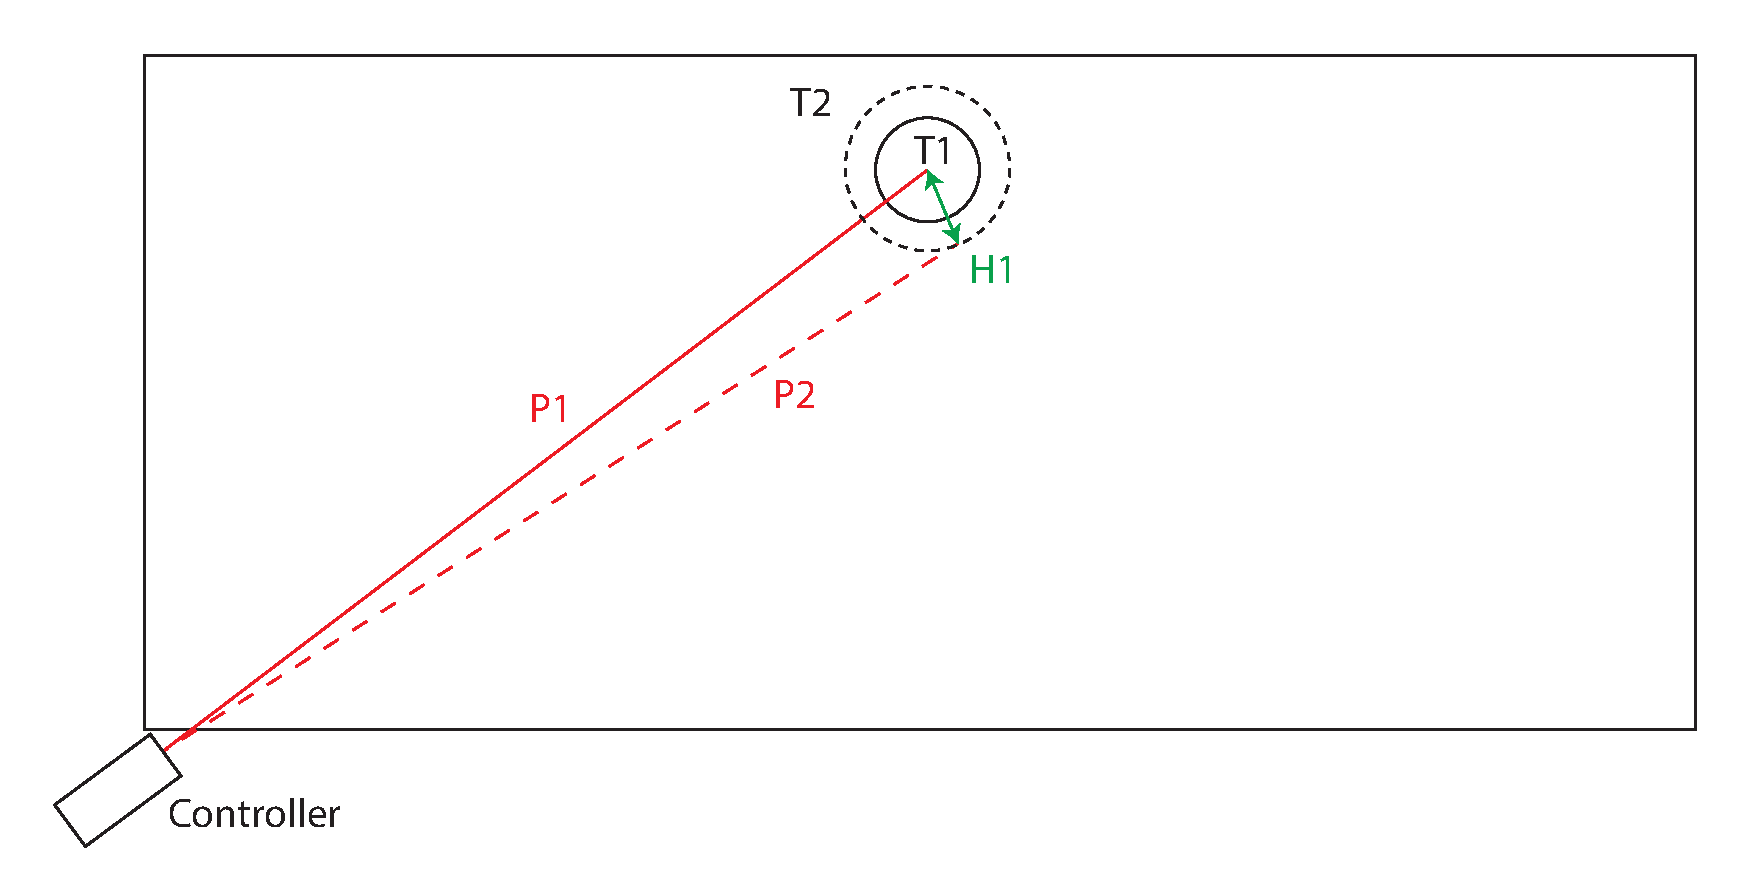
\includegraphics[width=.7\columnwidth]{graphics/heisenberg_effect_compensated.pdf}
    \caption{Possible Compensation for the Heisenberg Effect}
    \label{fig:heisenberg_effect_compensated}
\end{figure}

Because the ``Heisenberg Effect'' shows a similar range of effect on different modalities (like shown in Figure~\ref{fig:difference_handjitter_offset}), there is a chance, this effect can be predicted and measured. If this is, in an efficient algorithm and time possible, the effect could be canceled out in real life applications. For future work, it would be interesting to analyze the ``Heisenberg Effect'' in more real-life applications. A possible way to implement this, was already given by MacKenzie in his work on an extended Fitt's Law (described in subsection~\ref{subsec:related-work:background:extended_fitts_law})~\cite{mackenzie_extending_1992}: With enough data, it is possible to calculate if the user \textbf{wanted} to hit the target, more than if he really did. The software could now count a target as clicked on or hit, even if the user didn't hit it directly. Future work would have to take in consideration, that the created lag, caused by this additional computing time, could also have an effect on the performance of the user, like suggested by Pavlovych and Stuerzlinger~\cite{pavlovych_tradeoff_2009}.

The Figure~\ref{fig:heisenberg_effect_compensated} shows such a possible situation. The user wants to click on the target (T1) and aims the controller on this target (Line P1). Based on the disturbance in pointing made through the click (Line P2), the system would not detect this click, as one in the target. Because the ``Heisenberg Effect'' can be plotted over time, the system could now detect, that the user wanted to hit a target, a little bigger than the actual target (bigger target labeled as T2). Now the click is in the expanded target and the click would count.

One problem with the ``Heisenberg Effect'' wasn't cleared already and could be a topic for future work: The decrease of pointing accuracy could have an effect on the throughput. This aspect of the ``Heisenberg Effect'' wasn't discussed in this work. To sum up this work: it is clear that the effect needs to be farther researched, but a good base is given here.

\section{Acknowledgements}
Special thanks to Dennis Wolf for his help and advice in creating this thesis. 